\begin{frame}{Discrimination of Photon Added States}{Noisy PASS discrimination}
    \begin{columns}
        \begin{column}{0.5\linewidth}%<1->
            \begin{center}
                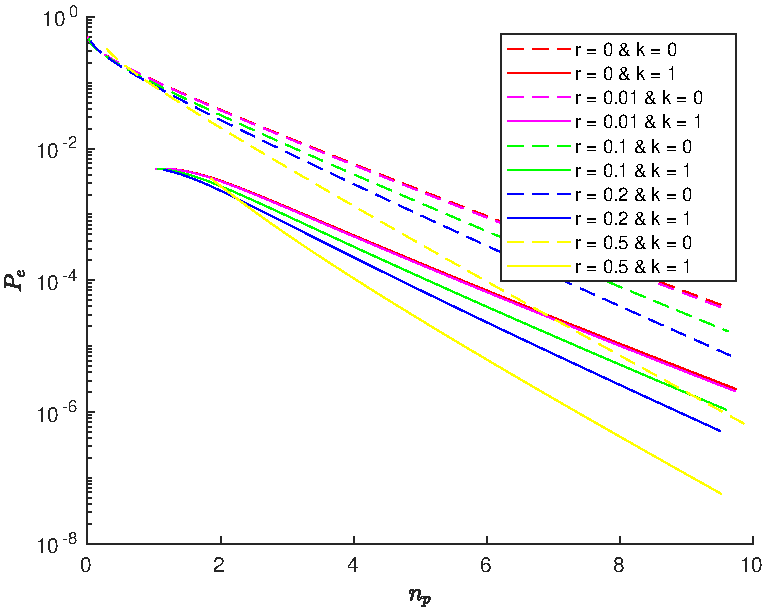
\includegraphics[width=1\textwidth]{Pictures/fig3.6.pdf}\\
                \scriptsize{
                MDEP of a QOOK system with PASS in terms of the mean photon number $n_p$.\\
                $N=30$; $\bar{n}=10^{-2}$; $\theta=\pi$; $p_0=p_1=1/2$
                }
            \end{center}
        %\end{frame}
        \end{column}
        
        \begin{column}{0.5\linewidth}%<2->
            %\begin{frame}{Discrimination of Photon Added States}{Noisy PASS discrimination: BPSK}
            \begin{center}
                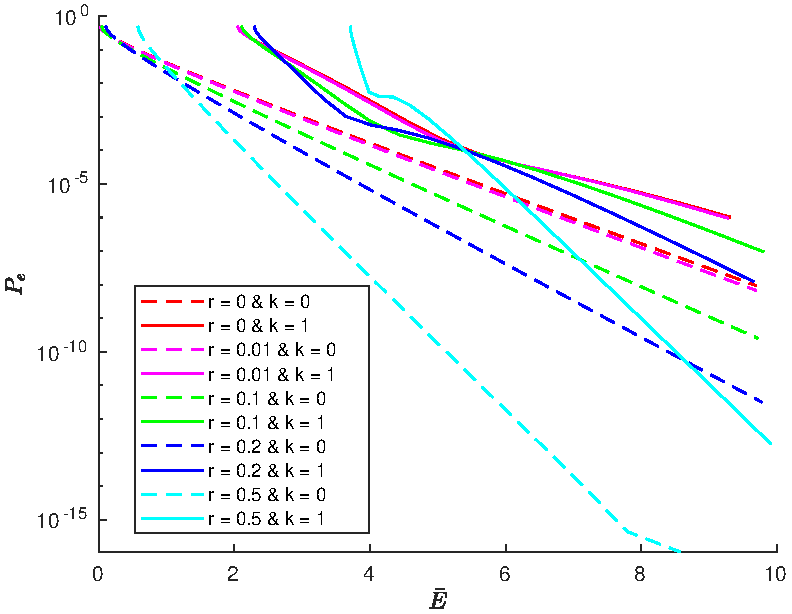
\includegraphics[width=1\textwidth]{Pictures/fig3.7.pdf}\\
                \scriptsize{
                MDEP of a QBPSK system with PASS in terms of the mean energy of the system $\bar{E}$.\\
                $N=30$; $\bar{n}=10^{-2}$; $\theta=\pi$; $p_0=p_1=1/2$
                }
            \end{center}
        \end{column}
    \end{columns}
\end{frame}  